
\de{ĐỀ THI HỌC KỲ I NĂM HỌC 2022-2023}{THPT Nguyễn Thái Bình}
\begin{center}
	\textbf{PHẦN 1 - TRẮC NGHIỆM}
\end{center}
\Opensolutionfile{ans}[ans/ans]

\begin{ex}%[0T3Y1-2]%[HKI-K10,Thehung Nguyen ]%[THPT NGUYEN THAI BÌNH]
Tập xác định $\mathscr{D}$ của hàm số $y=\sqrt{3x-1}$ là
\choice
{\True $\mathscr{D}=\left[\dfrac{1}{3};+\infty\right)$}
{$\mathscr{D}=\left(\dfrac{1}{3};+\infty\right)$}
{$\mathscr{D}=[0;+\infty)$}
{$\mathscr{D}=(0;+\infty)$}
\loigiai{
	Điều kiện xác định của hàm số $ 3x-1\ge 0\Leftrightarrow x\ge \dfrac{1}{3} $.\\
	Vậy tập xác định của hàm số là $\mathscr{D}=\left[\dfrac{1}{3};+\infty\right)$.
}
\end{ex}

\begin{ex}%[0T2Y1-1]%[HKI-K10,Thehung Nguyen ]%[THPT NGUYEN THAI BÌNH]
Bất phương trình nào sau đây là bất phương trình bậc nhất hai ẩn?
\choice
{\True $x+3y\le 2$}
{$(3x-y)(x+2y)\ge 5$}
{$y^3-2\le 0$}
{$x^2+y>3$}
\loigiai{
	Theo khái niệm của bất phương trình bậc nhất hai ẩn ta thấy trong các bất phương trình đã cho chỉ có bất phương trình $x+3y\le 2$ là bất phương trình bậc nhất hai ẩn.
}
\end{ex}
\begin{ex}%[0T5B4-6]%[HKI-K10,Thehung Nguyen ]%[THPT NGUYEN THAI BÌNH]
Cho $\overrightarrow{a}$ và $\overrightarrow{b}$ là hai véc-tơ đều khác véc-tơ $\overrightarrow{0}$ và có tích vô hướng bằng $ 0 $. Góc giữa hai véc-tơ này bằng
\choice
{$0^\circ$}
{$60^\circ$}
{\True $90^\circ$}
{$180^\circ$}
\loigiai{
	Theo định nghĩa tích vô hướng của hai véc-tơ ta có $$ \vec{a}.\vec{b}=|\vec{a}|\cdot |\vec{b}|\cdot \cos (\vec{a},\vec{b})=0\Rightarrow \cos (\vec{a},\vec{b})=0 \Rightarrow(\vec{a},\vec{b})=90^\circ .$$
}
\end{ex}
\begin{ex}%[0T4Y1-1]%[HKI-K10,Thehung Nguyen ]%[THPT NGUYEN THAI BÌNH]
Cho góc $\alpha$ là góc nhọn. Mệnh đề nào \textbf{sai} trong các mệnh đề sau?
\choice
{$\cot\alpha>0$}
{$\cos\alpha>0$}
{$\sin\alpha>0$}
{\True $\tan\alpha<0$}
\loigiai{
	Theo tính chất dấu của giá trị lượng giác ta có với $ \alpha $ nhọn thì $ \tan \alpha <0 $ là mệnh đề \textbf{sai}.
}
\end{ex}

\begin{ex}%[0T6Y1-1]%[HKI-K10,Thehung Nguyen ]%[THPT NGUYEN THAI BÌNH]
Cho số đúng $\overline{a}=1{,}49$ và số gần đúng $a=1{,}5$. Sai số tuyệt đối của số gần đúng $a$ là
\choice
{$ 0{,}1 $}
{$ 0{,}05 $}
{\True $ 0{,}01 $}
{$ 0{,}5 $}
\loigiai{
Sai số tuyệt đối $ \Delta_a=|a-\overline{a}| =|1{,5}-1{,}49|=0{,}01 $.
}
\end{ex}

\begin{ex}%[0T3Y2-2]%[HKI-K10,Thehung Nguyen ]%[THPT NGUYEN THAI BÌNH]
Hàm số nào sau đây là hàm số bậc hai?
\choice
{$y=2022x^3-5x+1$}
{\True $y=2x^2+x-2018$}
{$y=\dfrac{2x-1}{x+3}$}
{$y=-x^4+2$}
\loigiai{
	Theo khái niệm hàm số bậc hai ta thấy trong các đáp án trên thì $y=2x^2+x-2018$ là hàm số bậc hai.
}
\end{ex}
%
\begin{ex}%[0T5Y2-2]%[HKI-K10,Thehung Nguyen ]%[THPT NGUYEN THAI BÌNH]
Cho hình bình hành $ABCD$. Tìm véc-tơ $\overrightarrow{AB}+\overrightarrow{AD}-\overrightarrow{AC}$.
\choice
{$2\overrightarrow{AC}$}
{$-\overrightarrow{AC}$}
{$\overrightarrow{AC}$}
{\True $\overrightarrow{0}$}
\loigiai{
	Theo quy tắc hình bình hành ta có $ \overrightarrow{AB}+\overrightarrow{AD}= \overrightarrow{AC}$.\\
	Do đó $\overrightarrow{AB}+\overrightarrow{AD}-\overrightarrow{AC} =\vec{0}$.
}
\end{ex}
\begin{ex}%[0T2Y2-1]%[HKI-K10,Thehung Nguyen ]%[THPT NGUYEN THAI BÌNH]
Cặp số $(x;y)$ nào sau đây \textbf{không} là nghiệm của hệ bất phương trình $\heva{&3x+4y-1>0\\&x+2y-3\le 0}$?
\choice
{$(3;0)$}
{$(-1;2)$}
{\True $(0;0)$}
{$(2;0)$}
\loigiai{
	Thay tọa độ $ (0;0) $ vào hệ bất phương trình ta thấy $ \heva{&-1>0\text{ (vô lý)}\\&-3\le 0.} $\\
	Do đó $ (0;0) $ không là nghiệm của hệ bất phương trình đã cho.
}
\end{ex}
\begin{ex}%[0T3Y1-1]%[HKI-K10,Thehung Nguyen ]%[THPT NGUYEN THAI BÌNH]
Cho hàm số $f(x)=-3 x^2+2x-1$. Tính $f(2)$.
\choice
{$f(2)=-6$}
{\True $f(2)=-9$}
{$f(2)=0$}
{$f(2)=2$}
\loigiai{
	Ta có $ f(2)=-3\cdot 2^2+2\cdot 2-1=-9 $.
}
\end{ex}
\begin{ex}%[0T3Y1-1]%[HKI-K10,Thehung Nguyen ]%[THPT NGUYEN THAI BÌNH]
Điểm nào sau đây thuộc đồ thị hàm số $y=-x^2-2x+1$.
\choice
{$I(2;2)$}
{$M(1;0)$}
{$M(-3;6)$}
{\True $M(0;1)$}
\loigiai{
	Với $ x=0  $ thay vào hàm số  ta có $ y=1 $. Do đó $M(0;1)$ thuộc đồ thị hàm số $y=-x^2-2x+1$.
}
\end{ex}



\begin{ex}%[Đề THPT Nguyễn Thái Bình]%[Nguyễn Tài Tuệ]%[0T5Y1-1]
Từ hai điểm phân biệt $A,B$ xác định được bao nhiêu vectơ khác $\overrightarrow{0}$?
\choice
{$4$}
{\True $2$}
{$1$}
{$3$}
\loigiai{
	Có hai véc-tơ khác $\overrightarrow{0}$ có điểm đầu là điểm cuối là hai điểm phân biệt $ A $, $ B $ là $ \overrightarrow{AB} $, $ \overrightarrow{BA} $.
}
\end{ex}
\begin{ex}%[Đề THPT Nguyễn Thái Bình]%[Nguyễn Tài Tuệ]%[0T5Y2-1]
Cho các điểm phân biệt $A,B,C$. Đẳng thức nào sau đây \textbf{đúng}?
\choice
{$\overrightarrow{AB}=\overrightarrow{BC}+\overrightarrow{CA}$}
{\True $\overrightarrow{AB}=\overrightarrow{AC}+\overrightarrow{CB}$}
{$\overrightarrow{AB}=\overrightarrow{BC}+\overrightarrow{AC}$}
{$\overrightarrow{AB}=\overrightarrow{CA}+\overrightarrow{CB}$}
\loigiai{
	Theo quy tắc cộng véc-tơ ta có  $\overrightarrow{AB}=\overrightarrow{AC}+\overrightarrow{CB}$.
}
\end{ex}
\begin{ex}%[Đề THPT Nguyễn Thái Bình]%[Nguyễn Tài Tuệ]%[0T3B2-4]
Tọa độ giao điểm của parabol $(P)\colon y=x^2+5x+4$ với trục hoành là
\choice
{$(0;-1);(-4;0)$}
{$(-1;0);(0;-4)$}
{\True $(-1;0);(-4;0)$}
{$(0;-1);(0;-4)$}
\loigiai{
Hoành độ giao điểm  là nghiệm của phương trình $ x^2+5x+4=0\Leftrightarrow \hoac{&x=-1\\&x=-4.} $\\
Vậy tọa độ giao điểm của parabol $(P)\colon y=x^2+5x+4$ với trục hoành là  $(-1;0)$, $(-4;0)$.
}
\end{ex}
\begin{ex}%[Đề THPT Nguyễn Thái Bình]%[Nguyễn Tài Tuệ]%[0T4B2-1]
Cho tam giác $ABC$ có $a=5$, $A=60^\circ$. Tính bán kính đường tròn ngoại tiếp tam giác $ABC$.\\
\choice
{$\dfrac{5}{3}$}
{\True $\dfrac{5\sqrt{3}}{3}$}
{$\dfrac{10\sqrt{3}}{3}$}
{$5\sqrt{3}$}
\loigiai{
	Theo định sin ta có $ \dfrac{a}{\sin A } =2R \Rightarrow R=\dfrac{a}{2\sin  A}=\dfrac{5}{\sqrt{3}}.$
}
\end{ex}
\begin{ex}%[Đề THPT Nguyễn Thái Bình]%[Nguyễn Tài Tuệ]%[0T3Y2-2]
Cho hàm số $y=a x^2+b x+c(a\ne 0)$ có đồ thị $(P)$. Tọa độ đỉnh của $(P)$ là
\choice
{\True $I\left(-\dfrac{b}{2a};-\dfrac{\Delta}{4a}\right)$}
{$I\left(-\dfrac{b}{2a};\dfrac{\Delta}{4a}\right)$}
{$I\left(\dfrac{b}{2a};\dfrac{\Delta}{4a}\right)$}
{$I\left(-\dfrac{b}{a};-\dfrac{\Delta}{4a}\right)$}
\loigiai{
	Tọa độ đỉnh của parabol là $I\left(-\dfrac{b}{2a};-\dfrac{\Delta}{4a}\right)$.
}
\end{ex}
\begin{ex}%[Đề THPT Nguyễn Thái Bình]%[Nguyễn Tài Tuệ]%[0T6B3-1]
Bảng thống kê số lớp và số học sinh theo từng khối ở một trường THPT.
\begin{center}
\begin{tabular}{|l|c|c|c|}
\hline
Khối&10&11&12\\
\hline
Số lớp&12&13&12\\
\hline
Số học sinh&385&553&470\\
\hline
\end{tabular}
\end{center}
Hiệu trưởng trường đó cho biết sĩ số học sinh của mỗi lớp lớn hơn $ 30 $ và không vượt quá $ 40 $ em. Khối lớp bị thống kê sai là
\choice
{Khối $ 10 $}
{\True Khối $ 11 $}
{Khối $ 10 $, $ 12 $}
{Khối $ 12 $}
\loigiai{
	Số học sinh trung bình của khối $ 10 $ là $ \overline{x}_1=\dfrac{385}{12}\approx 32,09 $.\\
	Số học sinh trung bình của khối $ 11 $ là $ \overline{x}_2=\dfrac{553}{13}\approx 42,54 $.\\
	Số học sinh trung bình của khối $ 12$ là $ \overline{x}_3=\dfrac{470}{12}\approx 39,17 $.\\
	Theo thống kê trung bình trên thì ta thấy số học sinh trung bình khối 11 đang lớn hơn $ 40 $ nên khối 11 bị thống kê sai.
}
\end{ex}
\begin{ex}%[Đề THPT Nguyễn Thái Bình]%[Nguyễn Tài Tuệ]%[0T4Y2-1]
Cho tam giác $ABC$ có $BC=a,AC=b$ và $AB=c$. Khẳng định nào sau đây \textbf{đúng}?
\choice
{$\cos A=\dfrac{b^2+c^2+a^2}{b c}$}
{\True $\cos A=\dfrac{b^2+c^2-a^2}{2b c}$}
{$\cos A=\dfrac{b^2+c^2-a^2}{b c}$}
{$\cos A=\dfrac{b^2+c^2+a^2}{2b c}$}
\loigiai{
	Theo định lí cô-sin ta có $\cos A=\dfrac{b^2+c^2-a^2}{2b c}$.
}
\end{ex}
\begin{ex}%[Đề THPT Nguyễn Thái Bình]%[Nguyễn Tài Tuệ]%[0T3Y2-3]
Cho bảng biến thiên của hàm số $y=f(x)$
\begin{center}

\begin{tikzpicture}[>=stealth]
\tkzTabInit[nocadre=false,lgt=1,espcl=4,deltacl=0.5]{$x$/.7 ,$y$/2}
{$-\infty$ , $1$ , $+\infty$}
\tkzTabVar{+/$+\infty$ , -/$1$ , +/$+\infty$}
\end{tikzpicture}
\end{center}
Hàm số nào sau đây có bảng biến thiên như trên?
\choice
{$y=-x^2+2x+1$}
{$y=x^2+1$}
{$y=-x^2-1$}
{\True $y=x^2-2x+2$}
\loigiai{
	Dựa vào bảng biến thiên ta thấy \begin{itemize}
		\item Parabol có bề lõm quay lên trên nên $ a>0 $.
		\item Parabol có tọa độ đỉnh $ I(1;1) $.
	\end{itemize}
Do đó parabol thỏa mãn yêu cầu bài toán là $y=x^2-2x+2$.
}
\end{ex}
\begin{ex}%[Đề THPT Nguyễn Thái Bình]%[Nguyễn Tài Tuệ]%[0T3B1-4]
\immini
{
Cho hàm số $y=f(x)$ xác định trên đoạn $[-3;2]$ và có đồ thị như hình vẽ bên. Khẳng định nào dưới đây là khẳng định \textbf{đúng}?
\choice
{Hàm số nghịch biến trên khoảng $(-3;-1)$}
{Hàm số nghịch biến trên khoảng $(1;2)$}
{\True Hàm số nghịch biến trên khoảng $(-1;1)$}
{Hàm số đồng biến trên khoảng $(-1;1)$}
}
{
\begin{tikzpicture}[line join = round, line cap = round,>=stealth,font=\footnotesize,scale=0.7]
\def\xt{-4}\def\xp{3}\def\yd{-2}\def\yt{5}
\draw[->] (\xt,0)--(\xp,0) node[below]{$x$};
\draw[->] (0,\yd)--(0,\yt) node[left]{$y$};
\draw[thick] (-3,2)--(-1,4);
\draw[thick] plot[domain=-1:2,samples=200,smooth](\x,{(\x-1)^2});
\draw[dashed] (-3,0) node[below]{$-3$}|-(0,2) node[right]{$2$} (-1,0) node[below]{$-1$}|-(0,4) node[right]{$4$} (2,0) node[below]{$2$}|-(0,1) (1,0) node[below]{$1$};
\fill (0,0) circle (1.5pt) node[below left]{$O$};
\end{tikzpicture}
}
\loigiai{
	Dựa vào đồ thị ta thấy hàm số đồng biến trên khoảng $ (-3;-1) $ và $ (1;2) $, nghịch biến trên khoảng $ (-1;1) $.
}
\end{ex}

\begin{ex}%[Đề THPT Nguyễn Thái Bình]%[Nguyễn Tài Tuệ]%[0T1Y2-1]
Cho tập hợp $A=\{x\in\mathbb{N}\mid x<4\}$. Tìm mệnh đề \textbf{đúng}?
\choice
{\True $A=\{0;1;2;3\}$}
{$A=\{1;2;3\}$}
{$A=\{0;1;2;3;4\}$}
{$A=\{4\}$}
\loigiai{
	 Ta có $A=\{x\in\mathbb{N}\mid x<4\}=\{0;1;2;3\}$. 
}
\end{ex}

\begin{ex}%[0T2Y1-2]%[Đề kiểm tra HKI - THPT Nguyễn Thái Bình]%[Tín Đạt Trần]
Cặp số nào sau đây là nghiệm của bất phương trình $2x-y+1<0$?
\choice
{$(3;5)$}
{$(0;-1)$}
{\True $(1;4)$}
{$(2;-1)$}
\loigiai{
Ta có $2\cdot 1-4+1=-1<0$ nên $(1;4)$ là nghiệm của bất phương trình $2x-y+1<0$.
}
\end{ex}

\begin{ex}%[0T1Y2-3]%[Đề kiểm tra HKI - THPT Nguyễn Thái Bình]%[Tín Đạt Trần]
Cho tập hợp $A=\left\{x\in\mathbb{R}\  \middle| \ 2x+6\ge 0\right\}$. Tìm mệnh đề \textbf{đúng}?
\choice
{$A=(-\infty;-3]$}
{$A=(-\infty;-3)$}
{\True $A=[-3;+\infty)$}
{$A=(-3;+\infty)$}
\loigiai{
Ta có $2x+6\ge 0\Leftrightarrow 2x\ge -6\Leftrightarrow x\ge -3$.\\
Vậy $A=[-3;+\infty)$.
}
\end{ex}

\begin{ex}%[0T6Y1-2]%[Đề kiểm tra HKI - THPT Nguyễn Thái Bình]%[Tín Đạt Trần]
Số quy tròn của số gần đúng $a=2{,}235$ với độ chính xác $d=0{,}002$ là
\choice
{$2{,}2$}
{$2{,}23$}
{$2{,}235$}
{\True $2{,}24$}
\loigiai{
Hàng của chữ số $0$ đầu tiên bên trái của $d=0{,}002$ là hàng phần trăm nên số quy tròn đến hàng phần trăm của $a=2{,}235$ là $2{,}24$.
}
\end{ex}

\begin{ex}%[0T2B2-3]%[Đề kiểm tra HKI - THPT Nguyễn Thái Bình]%[Tín Đạt Trần]
\immini
{
Cho miền nghiệm (phần không gạch chéo) của bất phương trình bậc nhất hai ẩn như hình vẽ. Bất phương trình nào sau đây nhận miền nghiệm trên làm tập nghiệm?
\choice
{\True $2x+3y<8$}
{$3x+2y>8$}
{$3x+2y<8$}
{$2x+3y>8$}
}
{
\begin{tikzpicture}[line join=round, line cap=round,>=stealth,thick]
\tikzset{every node/.style={scale=0.7}}
\begin{scope}
\clip (-4,-1) rectangle (5,5);
%\fill[black!35] (-5,11.5)--(6,11.5)--(6,-5)--cycle;
\fill[pattern=north east lines] (-5,6)--(6,6)--(6,-1.33)--cycle;
%\draw (-0.67,5)--(3.33,-1) node [pos=0.45, above, sloped] {$3x+2y-8=0$};
\draw (-3.5,5)--(5.5,-1);
\end{scope}
\draw[->] (-4,0)--(5,0) node[below]{$x$};
\draw[->] (0,-1)--(0,5) node[left]{$y$};
\draw (0,0) node[below left]{$O$};
\foreach \x in {-3,-2,-1,1,2,3,4}
\draw[thin] (\x,1pt)--(\x,-1pt) node [below] {$\x$};
\foreach \y in {1,2,3,4}
\draw[thin] (1pt,\y)--(-1pt,\y) node [left] {$\y$};
\end{tikzpicture}
}
\loigiai{
Dựa vào đồ thị, ta có biên của miền nghiệm là đường thẳng $2x+3y=8$.\\
Điểm $O(0;0)$ thuộc miền nghiệm của bất phương trình đã cho nên bất phương trình đó là $2x+3y<0$.
}
\end{ex}

\begin{ex}%[0T4Y2-1]%[Đề kiểm tra HKI - THPT Nguyễn Thái Bình]%[Tín Đạt Trần]
Tam giác $ABC$ có $a=8$, $c=3$, $\widehat{B}=60^\circ$. Độ dài cạnh $b$ bằng bao nhiêu?
\choice
{$49$}
{$\sqrt{97}$}
{$\sqrt{61}$}
{\True $7$}
\loigiai{
Tam giác $ABC$ có $b^2=a^2+c^2-2ac\cos B=8^2+3^2-2\cdot 8\cdot 3\cdot \cos 60^\circ=49\Rightarrow b=7$.
}
\end{ex}
\begin{ex}%[0T1B3-1]%[Đề kiểm tra HKI - THPT Nguyễn Thái Bình]%[Tín Đạt Trần]
Cho hai tập hợp $A=[-5;3)$, $B=(1;+\infty)$. Khi đó $A\cap B$ là tập nào sau đây?
\choice
{$(1;3]$}
{\True $(1;3)$}
{$[5;+\infty)$}
{$[-5;1]$}
\loigiai{
Ta có $x\in A\cap B\Leftrightarrow \heva{&-5\leq x< 3\\&x>1}\Leftrightarrow 1<x<3$.\\
Suy ra $A\cap B=(1;3)$.
}
\end{ex}

\begin{ex}%[0T6Y2-2]%[Đề kiểm tra HKI - THPT Nguyễn Thái Bình]%[Tín Đạt Trần]
Tỷ lệ phần trăm về hạnh kiểm của học sinh trường $A$ được biểu diễn bởi biểu đồ sau:
\begin{center}
\newcommand{\chuthichbieudo}[2][]{
\begin{tikzpicture}
\def \canhhv{0.4}
\fill[#1] (0,0) rectangle (\canhhv,\canhhv);
\path (\canhhv,0)--(\canhhv,\canhhv) node[midway,right]{#2};
\end{tikzpicture}
}
\begin{tikzpicture}[line join = round, line cap = round,>=stealth,font=\footnotesize,scale=1]
\def \r{2}
\def \kc{0.5}
\def \mau{{"north east lines","grid","north west lines","horizontal lines"}}
\def \tile{{"43.8","49.1","5","2.1"}}
\def \ghichu{{"Khá","Tốt","Trung bình","Yếu"}}
\coordinate (O) at (0,0);
\pgfmathsetmacro{\curA}{90}
\foreach \i in {0,1,2,3}
{
\pgfmathsetmacro{\tileve}{\tile[\i]}
\pgfmathsetmacro{\mauve}{\mau[\i]}
\pgfmathsetmacro{\ghichuve}{\ghichu[\i]}
%\definecolor{mau\i}{HTML}{\mauve}
\pgfmathsetmacro{\deltaA}{\tileve/100*360}
\pgfmathsetmacro{\nextA}{\curA - \deltaA}
\pgfmathsetmacro{\midA}{(\curA+\nextA)/2}
\fill[pattern=\mauve,draw=white] (O)-- +(\curA:\r) arc (\curA:\nextA:\r) -- cycle;
%\node at ($(O)+(\midA:{\r+0.3})$)[align=center]{\tiny \ghichuve\\[-1ex]\tiny$\tileve\%$};
\node at ($($(O)+({\r+2},{\r-0.9})$)+(0,-\i*\kc)$)[right]{\chuthichbieudo[pattern=\mauve]{\ghichuve}};
\global\let\curA\nextA
}
\foreach \i in {0,1,2}
{
\pgfmathsetmacro{\tileve}{\tile[\i]}
\pgfmathsetmacro{\mauve}{\mau[\i]}
\pgfmathsetmacro{\ghichuve}{\ghichu[\i]}
%\definecolor{mau\i}{HTML}{\mauve}
\pgfmathsetmacro{\deltaA}{\tileve/100*360}
\pgfmathsetmacro{\nextA}{\curA - \deltaA}
\pgfmathsetmacro{\midA}{(\curA+\nextA)/2}
%\fill[pattern=\mauve,draw=white] (O)-- +(\curA:\r) arc (\curA:\nextA:\r) -- cycle;
\node at ($(O)+(\midA:{\r+0.3})$)[align=center]{\tiny \ghichuve\\[-1ex]\tiny$\tileve\%$};
%\node at ($($(O)+({\r+2},{\r-0.9})$)+(0,-\i*\kc)$)[right]{\chuthichbieudo[pattern=\mauve]{\ghichuve}};
\global\let\curA\nextA
}
\end{tikzpicture}
\end{center}
Số học sinh đạt hạnh kiểm yếu chiếm bao nhiêu phần trăm?
\choice
{$3,1\%$}
{$4\%$}
{$3\%$}
{\True $2,1\%$}
\loigiai{
Tỉ lệ phần trăm của số học sinh đạt hạnh kiểm yếu là $100\%-\left(43{,}8\%+49{,}1\%+5\%\right)=2{,}1\%$.
}
\end{ex}

\begin{ex}%[0T3B2-2]%[Đề kiểm tra HKI - THPT Nguyễn Thái Bình]%[Tín Đạt Trần]
\immini
{
Parabol dưới đây là đồ thị của hàm số nào?
\choice
{$y=-x^2-2x+1$}
{$y=x^2-2x-1$}
{\True $y=x^2+2x-1$}
{$y=-2x^2+2x-1$}
}
{
\begin{tikzpicture}[line join = round, line cap = round,>=stealth,font=\footnotesize,scale=1,declare function={f(\x)=(\x)^2+2*(\x)-1;}]
\def\xt{-3.5} \def\xp{2} \def\yd{-3} \def\yt{1.5}
\draw[->] (\xt,0)--(\xp,0) node[below]{$x$};
\draw[->] (0,\yd)--(0,\yt) node[left]{$y$};
\fill (0,0) circle (1.5pt) node[below left]{$O$};
\begin{scope}
\clip (\xt+0.1,\yd+0.1) rectangle (\xp-0.1,\yt-0.1);
\draw[samples=200,domain=\xt:\xp,smooth] plot (\x, {f(\x)});
\end{scope}
\draw[dashed] (-1,0)|-(0,-2);
\foreach \hoanh/\goc in {-1/90,-2/90} \fill (\hoanh,0) circle (1.5pt) ($(\hoanh,0)+(\goc:3.2mm)$) node{$\hoanh$};
\foreach \tung/\goc in {-1/0,-2/0} \fill (0,\tung) circle (1.5pt) ($(0,\tung)+(\goc:3.2mm)$) node{$\tung$};
\end{tikzpicture}
}
\loigiai{
Đặt $y=f(x)=ax^2+bx+c$.\\
Dựa vào đồ thị của hàm số, ta có 
\begin{eqnarray*}
	\heva{&\dfrac{-b}{2a}=-1\\&a\cdot \left(-1\right)^2+b\cdot \left(-1\right)+c=-2\\&a\cdot 0^2+b\cdot 0+c=-2}\Leftrightarrow \heva{&2a-b=0\\&a-b+c=-2\\&c=-1}\Leftrightarrow \heva{&a=1\\&b=2\\&c=-1.}
\end{eqnarray*}
Vậy $y=f(x)=x^2+2x-1$.
}
\end{ex}


\begin{ex}%[0T2B2-3]%[Đề kiểm tra HKI - THPT Nguyễn Thái Bình]%[Tín Đạt Trần]
\immini
{
Phần không tô đậm trong hình vẽ dưới đây (không chứa biên), biểu diễn tập nghiệm của hệ bất phương trình nào trong các hệ bất phương trình sau?
\choice
{$\heva{&x-y>0\\&2x-y<1}$}
{$\heva{&x-y<0\\&2x-y<1}$}
{$\heva{&x-y<0\\&2x-y>1}$}
{\True $\heva{&x-y>0\\&2x-y>1}$}
}
{
\begin{tikzpicture}[line join=round, line cap=round,>=stealth,thick]
\tikzset{every node/.style={scale=0.9}}
\begin{scope}
\clip (-2,-2.5) rectangle (3,3);
\fill[pattern=north east lines] (-3,-3)--(-3,4)--(4,4)--cycle;
\fill[pattern=north west lines] (-3,-7)--(-3,7)--(4,7)--cycle;
\draw (3,3)--(-2.5,-2.5);
\draw (2,3)--(-0.75,-2.5);
\end{scope}
\draw[->] (-2,0)--(3,0) node[below]{$x$};
\draw[->] (0,-2.5)--(0,3) node[left]{$y$};
\draw (0,0) node[below left,fill=white]{\color{black}$O$};
\foreach \x in {1}
\draw[thin] (\x,1pt)--(\x,-1pt) node [below] {$\x$};
\foreach \y in {1}
\draw[thin] (1pt,\y)--(-1pt,\y) node [left,fill=white] {\color{black}$\y$};
\draw[dashed,thin] (1,0)--(1,1)--(0,1);
\end{tikzpicture}
}
\loigiai{
Dựa vào hình vẽ, ta có hai biên là hai đường thẳng $x-y=0$ và $2x-y=1$.\\
Vì điểm $(1;0)$ nằm trong miền nghiệm của hệ bất phương trình đã cho nên hệ bất phương trình đó là $\heva{&x-y>0\\&2x-y>1.}$
}
\end{ex}


\begin{ex}%[0T4Y2-1]%[Đề kiểm tra HKI - THPT Nguyễn Thái Bình]%[Tín Đạt Trần]
Cho tam giác $ABC$ có $A=60^\circ$, $AB=7\mathrm{~cm}$, $AC=5\mathrm{~cm}$. Tính diện tích tam giác đã cho.
\choice
{$\dfrac{35\sqrt{3}}{2} \mathrm{~cm^2}$}
{\True $\dfrac{35\sqrt{3}}{4} \mathrm{~cm^2}$}
{$\dfrac{5\sqrt{3}}{4} \mathrm{~cm^2}$}
{$\dfrac{35\sqrt{3}}{2} \mathrm{~cm^2}$}
\loigiai{
Diện tích của tam giác đã cho là $S=\dfrac{1}{2}\cdot AB\cdot AC\cdot \sin A=\dfrac{1}{2}\cdot 7\cdot 5\cdot \sin 60^\circ=\dfrac{35\sqrt{3}}{4}\mathrm{~cm^2}$.
}
\end{ex}

%Câu 31...........................
\begin{ex}%[0T5Y2-1]%[Dự án đề kiểm tra HKII NH22-23- Nguyễn Sĩ Đạt]%[THPT Nguyễn Thái Bình]
Cho hình bình hành $ABCD$, giao điểm của hai đường chéo là $O$. Tìm mệnh đề \textbf{sai} trong các mệnh đề sau:
\choice
{$\vec{CO}-\vec{OB}=\vec{BA}$}
{$\vec{AB}-\vec{BC}=\vec{DB}$}
{$\vec{DA}-\vec{DB}=\vec{OD}-\vec{OC}$}
{\True $\vec{DA}+\vec{DB}+\vec{DC}=\vec{0}$}
\loigiai{
	\begin{center}
		\begin{tikzpicture}[>=stealth]
			\coordinate[label=above left:{$A$}] (A) at (2,3);
			\coordinate[label=below left:{$B$}] (B) at (0,0);
			\coordinate[label=below right:{$C$}] (C) at (5,0);
			\coordinate[label=above right:{$D$}] (D) at (7,3);
			\draw[black] (A)--(B)--(C)--(D)--(A) (A)--(C)  (B)--(D);
			\path[name path=ac] (A)--(C); 
			\path[name path=bd] (B)--(D); 
			\path[name intersections={of= ac and bd,by=O}];
			\draw[black] (O) node [below] {$O$};
			\foreach \diem in {A,B,C,D,O}	\fill[black] (\diem)circle(1.5pt);
		\end{tikzpicture}
	\end{center}
	\begin{itemize}
		\item Ta có $\vec{CO}-\vec{OB}=\vec{CO}+\vec{BO}=\vec{CO}+\vec{OD}=\vec{CD}=\vec{BA}$.
		\item Ta có $\vec{AB}-\vec{BC}=\vec{DC}-\vec{BC}=\vec{DB}$.
		\item Ta có $\vec{DA}-\vec{DB}=\vec{BA}=\vec{BO}+\vec{OA}=\vec{OD}+\vec{CO}=\vec{OD}-\vec{OC}$.
		\item Ta có $\vec{DA}+\vec{DB}+\vec{DC}=\vec{DB}+\vec{DB}=2\vec{DB} \ne \vec{0}$.
	\end{itemize}
}
\end{ex}

%Câu 32...........................
\begin{ex}%[0T3B1-4]%[Dự án đề kiểm tra HKII NH22-23- Nguyễn Sĩ Đạt]%[THPT Nguyễn Thái Bình]
	\immini{Cho hàm số $f(x)=ax+b$ có đồ thị như hình vẽ bên. Khẳng định nào sau đây là đúng. 
	\choice
	{$f(1)>f(-2023)$}
	{$f(2022)<f(2023)$}
	{\True $f(2022)>f(2023)$}
	{$f(1)<f(2023)$}}
	{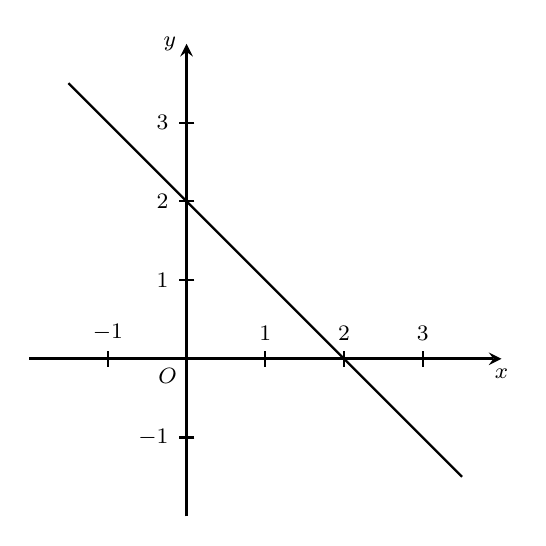
\begin{tikzpicture}[>=stealth,x=1cm,y=1cm,scale=1, font=\footnotesize]
			%%Vẽ trục tọa độ
			\draw[ line width=1,->] (-2,0) -- (4,0) node[below] {$x$};
			\draw[ line width=1,->] (0,-2) -- (0,4) node[left] {$y$};
			\draw (0,0)node[below left]{$O$};
			\foreach \x in {-1,1,2,...,3}\draw[line width=0.75] (\x,-0.1)--(\x,0.1) node [above] {\footnotesize $\x$};
			\foreach \y in {-1,...,-1,1,2,...,3}\draw[line width=0.75] (0.1,\y)--(-0.1,\y) node [left] {\footnotesize $\y$};	
			%%Khai báo hệ số a, b của hàm y=ax+b
			\def\a{-1}
			\def\b{2}
			%%Vẽ đồ thị (tự động dựa theo hệ số a, b đã nhập)
			\draw[thick,samples=150,smooth,domain=-1.5:3.5]%domain: vẽ đồ thị từ x=-2 đến x=4
			plot(\x,{\a*\x+(\b)});
	\end{tikzpicture}}
	\loigiai{
		Dựa vào đồ thị, suy ra $f(x)$ là hàm nghịch biến.\\
		Ta có: 
		\begin{itemize}
			\item $1>-2023 \Rightarrow f(1)<f(-2023)$.
		\item $2022<2023 \Rightarrow f(2022)>f(2023)$.
		\item $2022<2023 \Rightarrow f(2022)>f(2023)$.
		\item $1<2023 \Rightarrow f(1)>f(2023)$.
		\end{itemize}
	}
\end{ex}
%Câu 33...........................
\begin{ex}%[0T1B2-3]%[Dự án đề kiểm tra HKII NH22-23- Nguyễn Sĩ Đạt]%[THPT Nguyễn Thái Bình]
	Cho hai tập hợp $A=[-2;3)$ và $B=[m;m+5)$. Tìm tất cả các giá trị thực của tham số $m$ để $A\cap B\neq \emptyset$.
	\choice 
	{$-7<m\le -2$}
	{$-2<m\le 3$}
	{\True $-7<m<3$}
	{$-2\le m<3$}
	\loigiai
	{Ta có $A\cap B\neq \emptyset\Leftrightarrow \heva{&m<3\\&m+5>-2}\Leftrightarrow \heva{&m<3\\&m>-7}\Leftrightarrow -7<m<3$.}
\end{ex}
%Câu 34...........................

\begin{ex}%[0T4K3-1]%[Dự án đề kiểm tra HKII NH22-23- Nguyễn Sĩ Đạt]%[THPT Nguyễn Thái Bình]
	\immini{Hai trạm quan sát ở hai thành phố Đà Nẵng và Nha Trang đồng thời nhìn thấy một vệ tinh với góc nâng lần lượt là $75^\circ$ và $60^\circ$. Vệ tinh cách trạm quan sát tại thành phố Đà Nẵng $637$\,km. Khoảng cách giữa hai thành phố gần với giá trị nào sau đây?
	\choice
	{$510$\,km}
	{$530$\,km}
	{\True $520$\,km}
	{$540$\,km}}
	{\begin{tikzpicture}[font=\footnotesize,scale=1, line join=round, line cap=round, >=stealth] 
		\coordinate[label=below:$A$] (A) at (0,0);
		\coordinate[label=above:$C$] (C) at (1,3);
		\coordinate[label=below:$B$] (B) at (4,0);
		\draw[thick] (A)--(B)--(C)--(A)node[pos=.5, above left]{$637$ km};
		\draw pic["$75^{\circ}$", draw=black, angle eccentricity=1.6, angle radius=0.5cm]{angle=B--A--C};
		\draw pic["$60^{\circ}$", draw=black, angle eccentricity=1.6, angle radius=0.5cm]{angle=C--B--A};
		\end{tikzpicture}}
	\loigiai
	{Xét tam giác $ABC$ có $\widehat{A}+\widehat{B}+\widehat{C}=180^\circ\Rightarrow \widehat{C}=180^\circ-75^\circ-60^\circ=45^\circ$.\\
		Áp dụng định lí sin cho tam giác $ABC$, ta có
		\begin{center}
			$\dfrac{AB}{\sin{C}}=\dfrac{AC}{\sin{B}}\Rightarrow \dfrac{AB}{\sin{45^\circ}}=\dfrac{637}{\sin{60^\circ}}\Rightarrow AB=\dfrac{637\sqrt{6}}{3}\approx 520.$
		\end{center}
		Vậy khoảng cách giữa hai thành phố là khoảng $520$\,km.
	}
\end{ex}
%Câu 35...........................
\begin{ex}%[0T3B2-2]%[Dự án đề kiểm tra HKII NH22-23- Nguyễn Sĩ Đạt]%[THPT Nguyễn Thái Bình]
	Cho hàm số $y=-2x^2+bx+c$ có đồ thị là Parabol $(P)$ và có đỉnh $I(1;3)$. Khi đó $b+c$ bằng 
	\choice
	{$3$}{$4$}{$6$}{\True $5$}
	\loigiai{
		Do $I$ là đỉnh của $(P)$ nên ta có $x_I=\dfrac{-b}{2a} \Leftrightarrow 1=\dfrac{-b}{-4} \Leftrightarrow b=4$. \\
		Ta có $y_I=-2x_{I}^2+4x_{I}+c \Leftrightarrow c=1$. \\
		Vậy $b+c=5$.
	}
\end{ex}
%Câu 36...........................
\begin{ex}%[0T2K2-2]%[Dự án đề kiểm tra HKII NH22-23- Nguyễn Sĩ Đạt]%[THPT Nguyễn Thái Bình]
	Ông An dự định trồng lúa và khoai lang trên một mảnh đất có diện tích $10$ ha. Nếu trồng $1$ ha lúa thì cần 10 ngày công và thu được $20$ triệu đồng. Nếu trồng $1$ ha khoai lang thì cần $30$ ngày công và thu được $30$ triệu đồng. Biết rằng, ông An chỉ có thể sử dụng không quá $180$ ngày cho công việc trồng khoai lang và lúa. Số tiền nhiều nhất ông An thu được từ trồng hai loại cây nói trên là bao nhiêu?
	\choice
	{\True $240$ triệu đồng}
	{$180$ triệu đồng}
	{$260$ triệu đồng}
	{$200$ triệu đồng}
	\loigiai{
		Gọi $x$ là diện tích trồng lúa và $y$ là diện tích trồng khoai lang (đơn vị: ha, $x \ge 0, y\ge 0$).\\
		Theo đề bài, ta có hệ bất phương trình
		 \begin{center}
		 	$\heva{& 10x+30y \le 180\\ & x+y \le 10\\ & x \ge 0\\ &y \ge 0.} $
		 \end{center}
		Biểu diễn miền nghiệm của hệ bất phương trình này là miền tam giác $OABC$.
		\begin{center}
			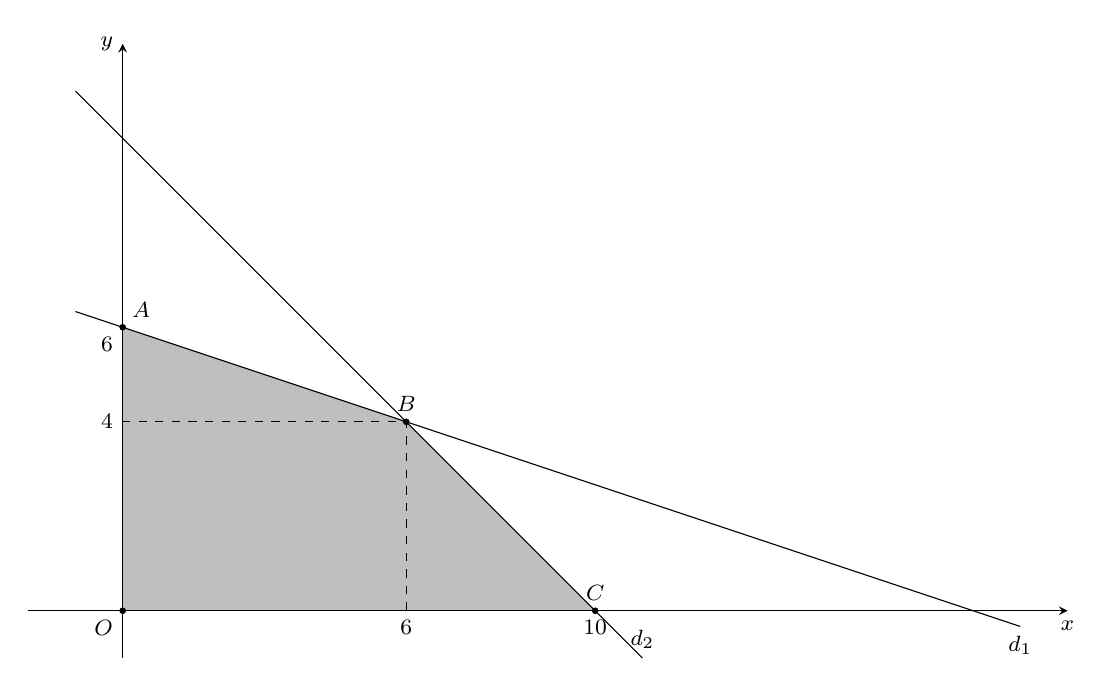
\begin{tikzpicture}[font=\footnotesize,>=stealth,x=1cm,y=1cm,scale=0.6]
				\coordinate[label=above right:$A$] (A) at (0,6); 
				\coordinate[label=above:$B$] (B) at (6,4); 
				\coordinate[label=above:$C$] (C) at (10,0); 
				\coordinate  (O) at (0,0);
				\fill[gray!50] (A)--(B)--(C)--(O)--(A);
				\draw[->] (-2,0) -- (20,0) node[below] {$x$};
				\draw[->] (0,-1) -- (0,12) node[left] {$y$};
				\fill (0,0)circle(2pt)node[below left]{$O$} (A)circle(2pt) (B)circle(2pt) (C)circle(2pt);
				\draw[dashed] (6,0)|-(0,4) ;
				\draw[samples=150,smooth,domain=-1:11] plot(\x,{(-1)*\x+(10)}) node[above]{$d_2$};
				\draw[samples=150,smooth,domain=-1:19] plot(\x,{(-1/3)*\x+(6)}) node[below]{$d_1$};
				\draw (10,0)node[below]{$10$} (6,0)node[below]{$6$} (0,4)node[left]{$4$} (0,6)node[below left]{$6$};
			\end{tikzpicture}
		\end{center}
		Tọa độ các đỉnh của tam giác đó: $O(0;0)$, $A(0;6)$, $B(6;4)$, $C(10;0)$.\\
		Gọi $F$ là số tiền ông An thu được (đơn vị: triệu đồng), khi đó $F=20x+30y$.\\
		Tại $O(0;0)$, ta có $F=20 \cdot 0 +30 \cdot 0=0$.\\
		Tại $A(0;6)$, ta có $F=20 \cdot 0 +30 \cdot 6=180$.\\
		Tại $B(6;4)$, ta có $F=20 \cdot 6 +30 \cdot 4=240$.\\
		Tại $C(10;0)$, ta có $F=20 \cdot 10 +30 \cdot 0=200$.\\
		Suy ra $F$ đạt giá trị lớn nhất bằng $240$ tại $B(6;0)$.\\
		Vậy số tiền nhiều nhất ông An thu được từ trồng hai loại cây nói trên là $240$ triệu đồng.
	}
\end{ex}
%Câu 37...........................
\begin{ex}%[0T2B2-3]%[Dự án đề kiểm tra HKII NH22-23- Nguyễn Sĩ Đạt]%[THPT Nguyễn Thái Bình]
	\immini{Cho hệ bất phương trình $\heva{&-2x+y \leq 2 \\ &-x+2y \geq 4 \\ &	x+y \leq 5}$ có miền nghiệm là miền được tô màu (miền tam giác $ABC$ có tọa độ các đỉnh là $A(0;2)$, $B(2;3)$, $C(1;4)$, bao gồm cả các cạnh như hình vẽ bên. Giá trị nhỏ nhất $F_{\min}$ của biểu thức $F(x;y)=-x+y$ trên miền xác định bởi hệ trên là
	\choice
	{$F_{\min}=4$}
	{$F_{\min}=3$}
	{\True $F_{\min}=1$}
	{$F_{\min}=2$}}
	{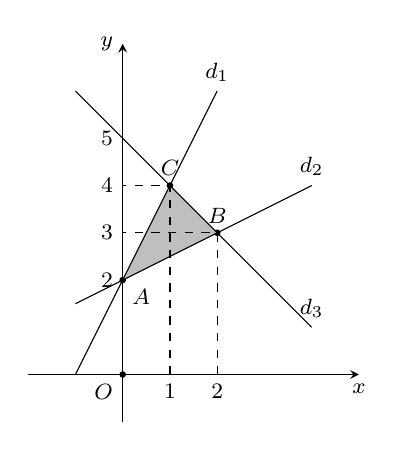
\begin{tikzpicture}[font=\footnotesize,>=stealth,x=1cm,y=1cm,scale=0.6]
			\coordinate[label=below right:$A$] (A) at (0,2); 
			\coordinate[label=above:$B$] (B) at (2,3); 
			\coordinate[label=above:$C$] (C) at (1,4); 
			\draw[->] (-2,0) -- (5,0) node[below] {$x$};
			\draw[->] (0,-1) -- (0,7) node[left] {$y$};
			\fill (0,0)circle(2pt)node[below left]{$O$} (A)circle(2pt) (B)circle(2pt) (C)circle(2pt);
			\fill[gray!50] (A)--(B)--(C)--(A);
			\draw[dashed] (2,0)|-(0,3) (1,0)|-(0,4);
			\draw[samples=150,smooth,domain=-1:4] plot(\x,{(.5)*\x+(2)}) node[above]{$d_2$};
			\draw[samples=150,smooth,domain=-1:4] plot(\x,{(-1)*\x+(5)}) node[above]{$d_3$};
			\draw[samples=150,smooth,domain=-1:2] plot(\x,{(2)*\x+(2)}) node[above]{$d_1$};
			\draw (1,0)node[below]{$1$} (2,0)node[below]{$2$} (0,2)node[left]{$2$} (0,3)node[left]{$3$} (0,4)node[left]{$4$} (0,5)node[left]{$5$};
	\end{tikzpicture}}
	\loigiai{
		Ta biết biểu thức $F(x;y)$ đạt giá trị nhỏ nhất tại các đỉnh của miền nghiệm $ABC$.\\
		Giá trị của $F$ tại các đỉnh của tam giác $ABC$:\\
		Tại $A(0;2) \colon F = -0 + 2 = 2$;\\
		Tại $B(2;3) \colon F = -2 + 3 = 1$;\\
		Tại $C(1;4) \colon F = -1 + 4 = 3$;\\
		Vậy $F_{\min}=1$ tại $B(2;3)$.
	}
\end{ex}
%Câu 38...........................
\begin{ex}%[0T2G2-2]%[Dự án đề kiểm tra HKII NH22-23- Nguyễn Sĩ Đạt]%[THPT Nguyễn Thái Bình]
Một xưởng sản xuất định lựa chọn hai loại máy chế biến loại I và loại II. Máy loại I mỗi ngày $1$ máy chế biến được $300$ kilogam sản phẩm, máy loại II mỗi ngày $1$ máy chế biến được $450$ kilogam sản phẩm. Biết để có lãi mỗi ngày xưởng phải sản xuất được nhiều hơn $50$ tấn sản phẩm. Hỏi xưởng nên lựa chọn số lượng máy như thế nào trong các phương án dưới đây để đảm bảo có lãi? 
\choice
{$80$ máy chế biến loại I và $50$ máy chế biến loại II}
{\True $50$ máy chế biến loại I và $80$ máy chế biến loại II}
{$65$ máy chế biến loại I và $65$ máy chế biến loại II}
{$70$ máy chế biến loại I và $60$ máy chế biến loại II}
\loigiai{
	Đổi $300$ kg $=0{,}3$ tấn; $450$ kg $=0{,}45$ tấn.\\
	Gọi $x$, $y$ (máy) lần lươt là số máy loại I và loại II $\left(x, y \leq 0\right)$ .\\
	Để đảm bảo có lãi thì $0{,}3x+0{,}45y>50$.\\
	Với đáp án A: $0{,}3 \cdot 80 + 0{,}45 \cdot 50 = 46{,}5 <50$ (loại).\\
	Với đáp án B: $0{,}3 \cdot 50 + 0{,}45 \cdot 80 = 52>50$ (nhận).\\
	Với đáp án C: $0{,}3 \cdot 65 + 0{,}45 \cdot 65 = 48{,}75 < 50$ (loại).\\
	Với đáp án D: $0{,}3 \cdot 70 + 0{,}45 \cdot 60 = 48 < 50$ (loại).
} 
\end{ex}
%Câu 39...........................
\begin{ex}%[0T5K4-1]%[Dự án đề kiểm tra HKII NH22-23- Nguyễn Sĩ Đạt]%[THPT Nguyễn Thái Bình]
Cho hình thoi $ABCD$ tâm $O$ có cạnh bằng $2a$ và góc $\widehat{ABD}$ bằng $60^\circ$. Gọi $I$ là điểm thỏa mãn $2\Vec{IC}+\Vec{ID}=\Vec{0}$. Tính tích vô hướng $\Vec{OI}\cdot\Vec{BI}.$ 
\choice
{$\vec{OI}\cdot\vec{BI}=-\dfrac{a^2}{4}$}
{$\vec{OI}\cdot\vec{BI}=\dfrac{a^2}{4}$}
{\True $\vec{OI}\cdot\vec{BI}=2a^2$}
{$\vec{OI}\cdot\vec{BI}=-a^2$}
\loigiai{
	\begin{center}
		\begin{tikzpicture}[scale=1.5, font=\footnotesize, line join=round, line cap=round, >=stealth,x=1cm,y=1cm] 
			\coordinate[label=below:$A$] (A) at (0,0);
			\coordinate[label=above:$B$] (B) at ($(A)+(30:2cm)$);
			\coordinate[label=below:$D$] (D) at ($(A)+(-30:2cm)$);
			\coordinate[label=below right:$O$] (O) at ($(B)!0.5!(D)$);  
			\coordinate[label=below:$C$] (C) at ($(A)!2!(O)$); 
			\coordinate[label=below:$I$] (I) at ($(C)!1/3!(D)$);   
			\draw (A)--(B)--(C)--(D)--(A)--(C) (I)--(B)--(D);
			\foreach \diem in {A,B,C,D,O,I}	\fill[black] (\diem)circle(1pt);
		\end{tikzpicture}
	\end{center}
	Vì $ABCD$ là hình thoi tâm $O$, $\widehat{ABD}=60^\circ$ nên tam giác $ABD$ đều.\\
	Suy ra: $AO = \dfrac{AB \sqrt{3}}{2} = a \sqrt{3}$.\\
	Ta có: 
	\begin{eqnarray*}
		2\Vec{IC}+\Vec{ID} =\Vec{0} 
		&\Leftrightarrow& 2 \vec{OC} - 2 \vec{OI} + \vec{OD} - \vec{OI} =\vec{0} \\ 
		&\Leftrightarrow& \vec{OI} = \dfrac{2}{3} \vec{OC} + \dfrac{1}{3} \vec{OD}.
	\end{eqnarray*}
	Khi đó:
	\begin{eqnarray*}
		\vec{AO}.\vec{BI} &=& \vec{AO}.\left(\vec{OI} - \vec{OB} \right)\\
		&=& \vec{AO}.\vec{OI} - \vec{AO}. \vec{OB}\\
		&=& \vec{AO}. \left(\dfrac{2}{3} \vec{OC} + \dfrac{1}{3} \vec{OD} \right) - 0\\
		&=& \dfrac{2}{3} \vec{AO}.\vec{OC} + \dfrac{1}{3} \vec{AO}.\vec{OD}\\
		&=& \dfrac{2}{3}AO^2 + 0\\
		&=& \dfrac{2}{3} \left(a \sqrt{3} \right)^2=2a^2.
	\end{eqnarray*}
} 
\end{ex}
%Câu 40...........................
\begin{ex}%[0T3G2-5]%[Dự án đề kiểm tra HKII NH22-23- Nguyễn Sĩ Đạt]%[THPT Nguyễn Thái Bình]
\immini{Một vật chuyển động trong $3$ giờ với vận tốc $v$ (km/h) phụ thuộc thời gian $t$ (h) có đồ thị là một phần của parabol có đinh là $I(2;9)$ và trục đối xứng song song với trục tung như hình vẽ. Vận tốc của vật tại thời điểm $2$ giờ $30$ phút sau khi vật bắt đầu chuyển động gần bằng giá trị nào nhất trong các giá trị sau đây? 
\choice
{$8{,}7$ (km/h)}
{$8{,}6$ (km/h)}
{\True $8{,}8$ (km/h)}
{$8{,}5$ (km/h)}}
{\begin{tikzpicture}[font=\footnotesize,>=stealth,x=1cm,y=1cm,scale=0.6]
		\def\a{-0.75} % Hệ số a phải khác 0
		\def\b{3}
		\def\c{6}
		\draw[->] (-5,0) -- (5,0) node[below] {$t$};
		\draw[->] (0,-1) -- (0,10) node[left] {$v$};
		\fill (0,0)circle(2pt)node[below left]{$O$} (2,9)circle(2pt)node[above]{$I$} (0,6)circle(2pt)node[left]{$6$}
		(0,9)circle(2pt)node[left]{$9$}
		(2,0)circle(2pt)node[below]{$2$}
		(3,0)circle(2pt)node[below]{$3$};
		\draw[dashed] (2,0)|-(0,9) (3,0)--(3,8.25);
		\draw[thick,samples=150,smooth,domain=0:3] plot(\x,{\a*(\x)^2+(\b)*\x+(\c)});
\end{tikzpicture}}
\loigiai{
Do vận tốc $v$ (km/h) phụ thuộc thời gian $t$ (h) có đồ thị là một phần của parabol nên ta gọi vận tốc của vật có phương trình chuyển động là $v(t)=at^2+bt+c$.\\
Theo đề bài, ta có
\begin{center}
	$\heva{&a\cdot 2^2+b\cdot 2+c = 9\\ &\dfrac{-b}{2a} = 2\\&a\cdot0+b\cdot 0+c = 6}\Leftrightarrow \heva{&4a+2b+c = 9\\ &4a+b=0\\&c = 6}\Leftrightarrow \heva{&4a=-\dfrac{3}{4}\\ &b=3\\&c = 6.}$
\end{center}
Suy ra $v(t)=-\dfrac{3}{4}t^2+3t+6$.\\
Ta có $2$ giờ $30$ = $2{,}5$ giờ.\\
Vậy $v(2{,}5)=\dfrac{- 3}{4}\cdot 2{,}5^2+3\cdot 2{,}5+6=8{,}125$ (km/h). 
}
\end{ex}


\Closesolutionfile{ans}
\begin{center}
	\textbf{ĐÁP ÁN}
	\inputansbox{10}{ans/ans}	
\end{center}
